\documentclass[border=10pt]{standalone}

\usepackage{tikz}
\usepackage{tikzsymbols}
\usetikzlibrary{calc,patterns,shapes.geometric}

\def\centerarc[#1](#2)(#3:#4:#5){\draw[#1] ($(#2)+({#5*cos(#3)},{#5*sin(#3)})$) arc (#3:#4:#5);}

\begin{document}
	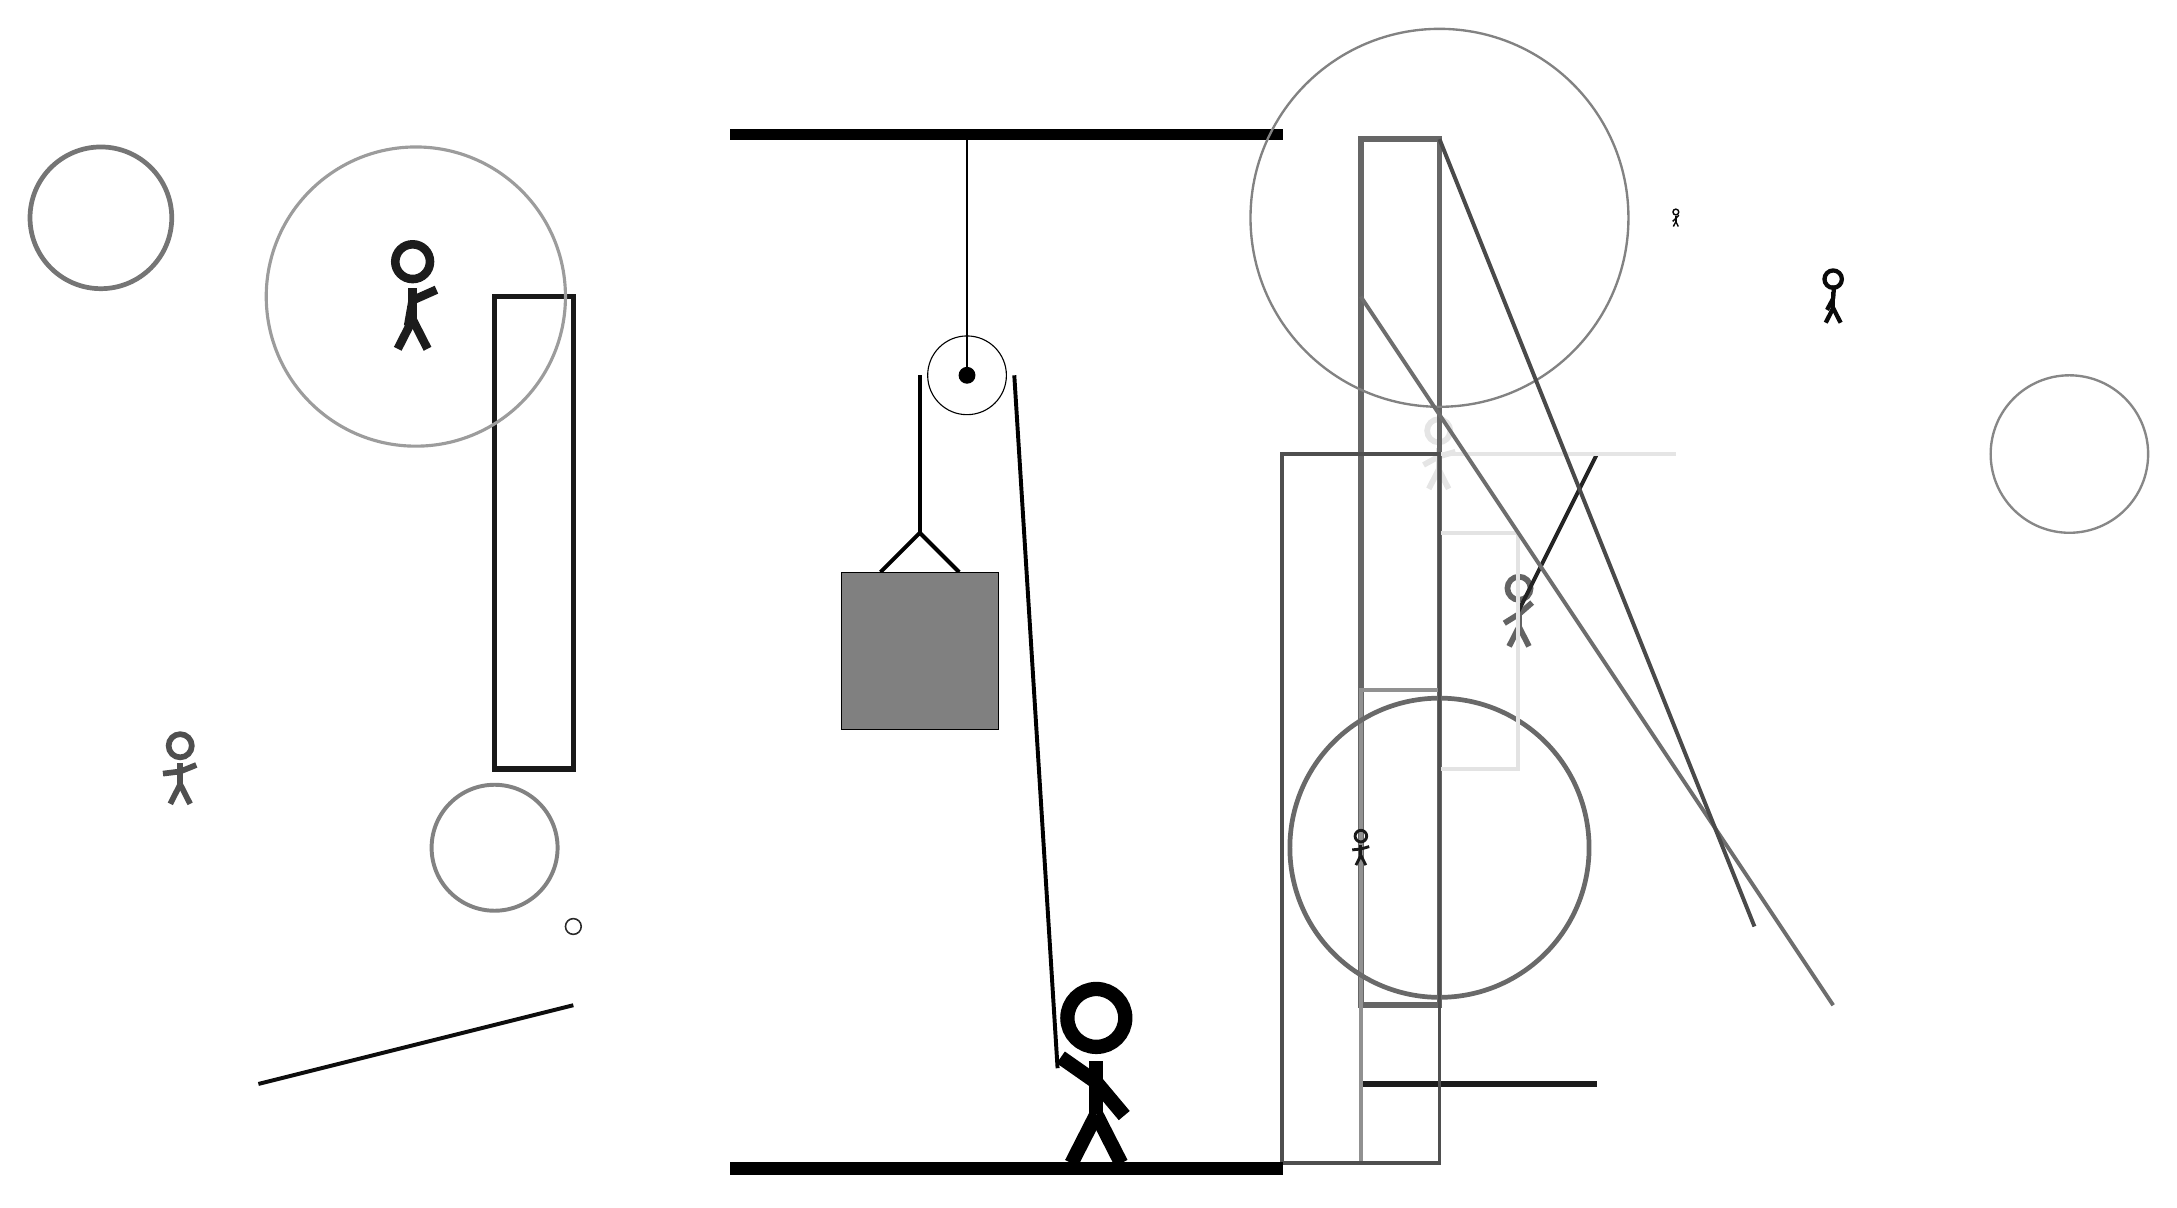
\begin{tikzpicture}
		%%%%% START %%%%%
		
		\draw[fill=black] (-2, 10) rectangle (5, 10.125);
		
		\draw (1, 7) circle (0.5);
		\draw[fill=black] (1, 7) circle (0.1);
		\draw (1, 10) -- (1, 7);
		
		\draw[line width=0.5mm] (-0.1, 4.5) -- (0.4, 5.0) -- (0.9, 4.5);
		\draw[fill=black!50] (-0.6, 4.5) rectangle (1.4, 2.5);
		
		\draw[line width=0.5mm] (0.4, 7) -- (0.4, 5.0);
		\centerarc[line width=0.5mm](1, 7)(0:180:0.6);
		\draw[line width=0.5mm](1.6, 7) -- (2.15, -1.8);
		
		\node[line width=0.6mm, color=black!97] at (10, 9) {\Strichmaxerl[1][42][48]};
		
		\draw[line width=0.4mm, color=black!16] (6, 10) rectangle (6, 6);
		\node[line width=0.4mm, color=black!69] at (-9, 2) {\Strichmaxerl[4][7][22]};
		\node[line width=0.6mm, color=black!96] at (12, 8) {\Strichmaxerl[3][62][86]};
		\draw [line width=0.5mm, color=black!49](-5, 1) circle (0.8);
		
		\draw[line width=0.7mm, color=black!89] (6, -2) rectangle (9, -2);
		
		\node[line width=0.2mm, color=black!10] at (7, 6) {\Strichmaxerl[4][29][16]};
		\draw [line width=0.6mm, color=black!54](-10, 9) circle (0.9);
		\draw[line width=0.7mm, color=black!90] (-4, 8) rectangle (-5, 2);
		
		\draw[line width=0.7mm, color=black!60] (6, -1) rectangle (7, 10);
		\draw [line width=0.2mm, color=black!84](-4, 0) circle (0.1);
		\node[line width=0.2mm, color=black!61] at (8, 4) {\Strichmaxerl[4][32][41]};
		\draw[line width=0.5mm, color=black!43] (7, -3) rectangle (6, 3);
		\draw[line width=0.5mm, color=black!86](9, 6) -- (8, 4);
		\node[line width=0.2mm, color=black!90] at (6, 1) {\Strichmaxerl[2][6][16]};
		\draw [line width=0.4mm, color=black!39](-6, 8) circle (1.9);
		
		\draw[line width=0.5mm, color=black!10](6, 6) -- (10, 6);
		\draw [line width=0.6mm, color=black!59](7, 1) circle (1.9);
		\draw[line width=0.2mm, color=black!60] (7, -1) rectangle (7, -1);
		
		\node[line width=0.5mm, color=black!89] at (-6, 8) {\Strichmaxerl[6][80][24]};
		\draw[line width=0.5mm, color=black!11] (7, 5) rectangle (8, 2);
		
		\draw [line width=0.3mm, color=black!49](7, 9) circle (2.4);
		\draw [line width=0.3mm, color=black!47](15, 6) circle (1.0);
		\draw[line width=0.5mm, color=black!57](6, 8) -- (12, -1);
		\draw[line width=0.5mm, color=black!69] (5, 6) rectangle (7, -3);
		
		\draw[line width=0.5mm, color=black!95](-4, -1) -- (-8, -2);
		\draw[line width=0.5mm, color=black!71](7, 10) -- (11, 0);
		
		\node at (2.6, -1.9) {\Strichmaxerl[10][-35][-50]};
		
		\draw[fill=black] (-2, -3) rectangle (5, -3.15);
		
		%%%%% END %%%%%
	\end{tikzpicture}
\end{document}